Because of the features of nonvolatile, very high density, and ultra-low power consumption, the emerging RRAM is believed to be a promising candidate for nonvolatile storage, in-memory computing, and neuromorphic applications. However, unstable device performance poses a challenge in reliable sensing and requires a special circuit structure for improving the sensing capability. 
An accurate RRAM circuit model including variations is also critical in designing a reliable sensing circuit. 

% The configuration of a one-transistor-one-RRAM (1T1R) cell is widely used in memory array design, in which one dedicated transistor controls the access of the RRAM device and complies the device current.

\subsection{RRAM Model and Simulation Framework}
\label{sim_model}
% An accuracy RRAM circuit model is the foundation of the study. 
In this work, we employ a simulation framework and the device models that are similar to \cite{9234102} and \cite{lu2020reram}. 
Table \ref{tab_model} summarizes key fundamental RRAM parameters that are used in our analysis. 
A commercial 40-nm standard CMOS design kit is utilized for transistors.
Post layout simulation and analysis are performed to optimize the design.


\begin{figure}[!t]
\centerline
{
\includegraphics[width=0.45\textwidth]{RRAM_IV_curve.pdf}}
\caption{The model simulation results of the RRAM DC I-V characteristic curves and read operation settings. The resistances of HRS and LRS are 500 K$\Omega$ and 10 K$\Omega$ respectively under the read voltage of 0.2 V.}
\label{IV_curve}
\end{figure}


\begin{table}[!t]
\centering
\caption{Key Parameters for Employed RRAM Device}
\label{tab_model}
 \begin{threeparttable}
% \begin{tabular}{|c{1.3cm}|p{1.5cm}|p{1.6cm}|p{1.3cm}|p{2cm}|p{1.3cm}|p{1.3cm}|p{5cm}|}
\begin{tabular}{@{}m{5cm}<{\centering}|m{2.5cm}<{\centering}@{}}
% \begin{tabular}{lllllll}
\toprule[1.5pt]
\hline
% This work & 65 & Differential, 4-stage  & 0.11-0.38\tnote{1}  & 80   \\\hline
RRAM size ($W\times L$)     & 100 nm $\times$ 100 nm  \\\hline
nominal resistance of HRS ($R_{HRS}$)   & 500 K$\Omega$  \\\hline
standard deviation of $R_{HRS}$   & 100 K$\Omega$  \\\hline
nominal resistance of LRS ($R_{LRS}$)  & 10 K$\Omega$  \\\hline
standard deviation of $R_{LRS}$   & 2 K$\Omega$  \\\hline
nominal set voltage ($V_{SET}$)        & 0.8 V  \\\hline
standard deviation of $V_{SET}$        & 0.15 V  \\\hline
nominal reset voltage ($V_{RESET}$)      & -1.1 V  \\\hline
standard deviation of $V_{RESET}$        & 0.225 V  \\\hline
read voltage ($V_{read}$)	& $0.2V$  \\\hline
temperature coefficient of $R_{HRS}$	& -0.0015  \\\hline
temperature coefficient of $R_{LRS}$	& 0.001  \\\hline
\bottomrule[1.5pt]
\end{tabular}
% \begin{tablenotes}
% \item[1] Excluding V-I converter power 
% \end{tablenotes}
\end{threeparttable}
\end{table} 
 

To restrain the sneak current of the half-selected cells, one common way to implement RRAM bit cells in an array is to integrate an RRAM device in series with a MOS transistor. This is known as the 1T1R structure \cite{6936923} where one dedicated transistor controls the access of the RRAM device and complies the device current.
Fig. \ref{IV_curve} shows the typical current-voltage (I-V) characteristic curves of an $HfO_x$ based RRAM with a cell size of $100\times 100$ nm$^2$. The red and blue curves represent HRS and LRS, respectively, whose resistances are 500 K and 10 K when the read voltage is 0.2 V. The left bottom of Fig. \ref{IV_curve} shows the read operation setting of the 1T1R bitcell while the right side illustrates the RRAM physical model at the LRS and HRS states. 
% The access transistor of 1T1R bitcell is a normal-VTH NMOS transistor with $W/L = 360nm/40nm$.

Cycle-to-cycle (C2C) and device-to-device (D2D) variations are statistically analyzed by Monte Carlo (MC) simulation using the RRAM model. For MOS transistors, both local and global variations are considered using the foundry model. It is assumed that the RRAM device parameters have Gaussian distribution for MC simulations, as listed in Table \ref{tab_model}. 
In each simulation iteration, MC analysis generates every parameter randomly according to the statistical distribution models of the RRAM device and the MOS transistors.
Corner analyses are also performed to guarantee the robustness of the design even in the worst case.



\begin{figure*}[!t]
\centerline
{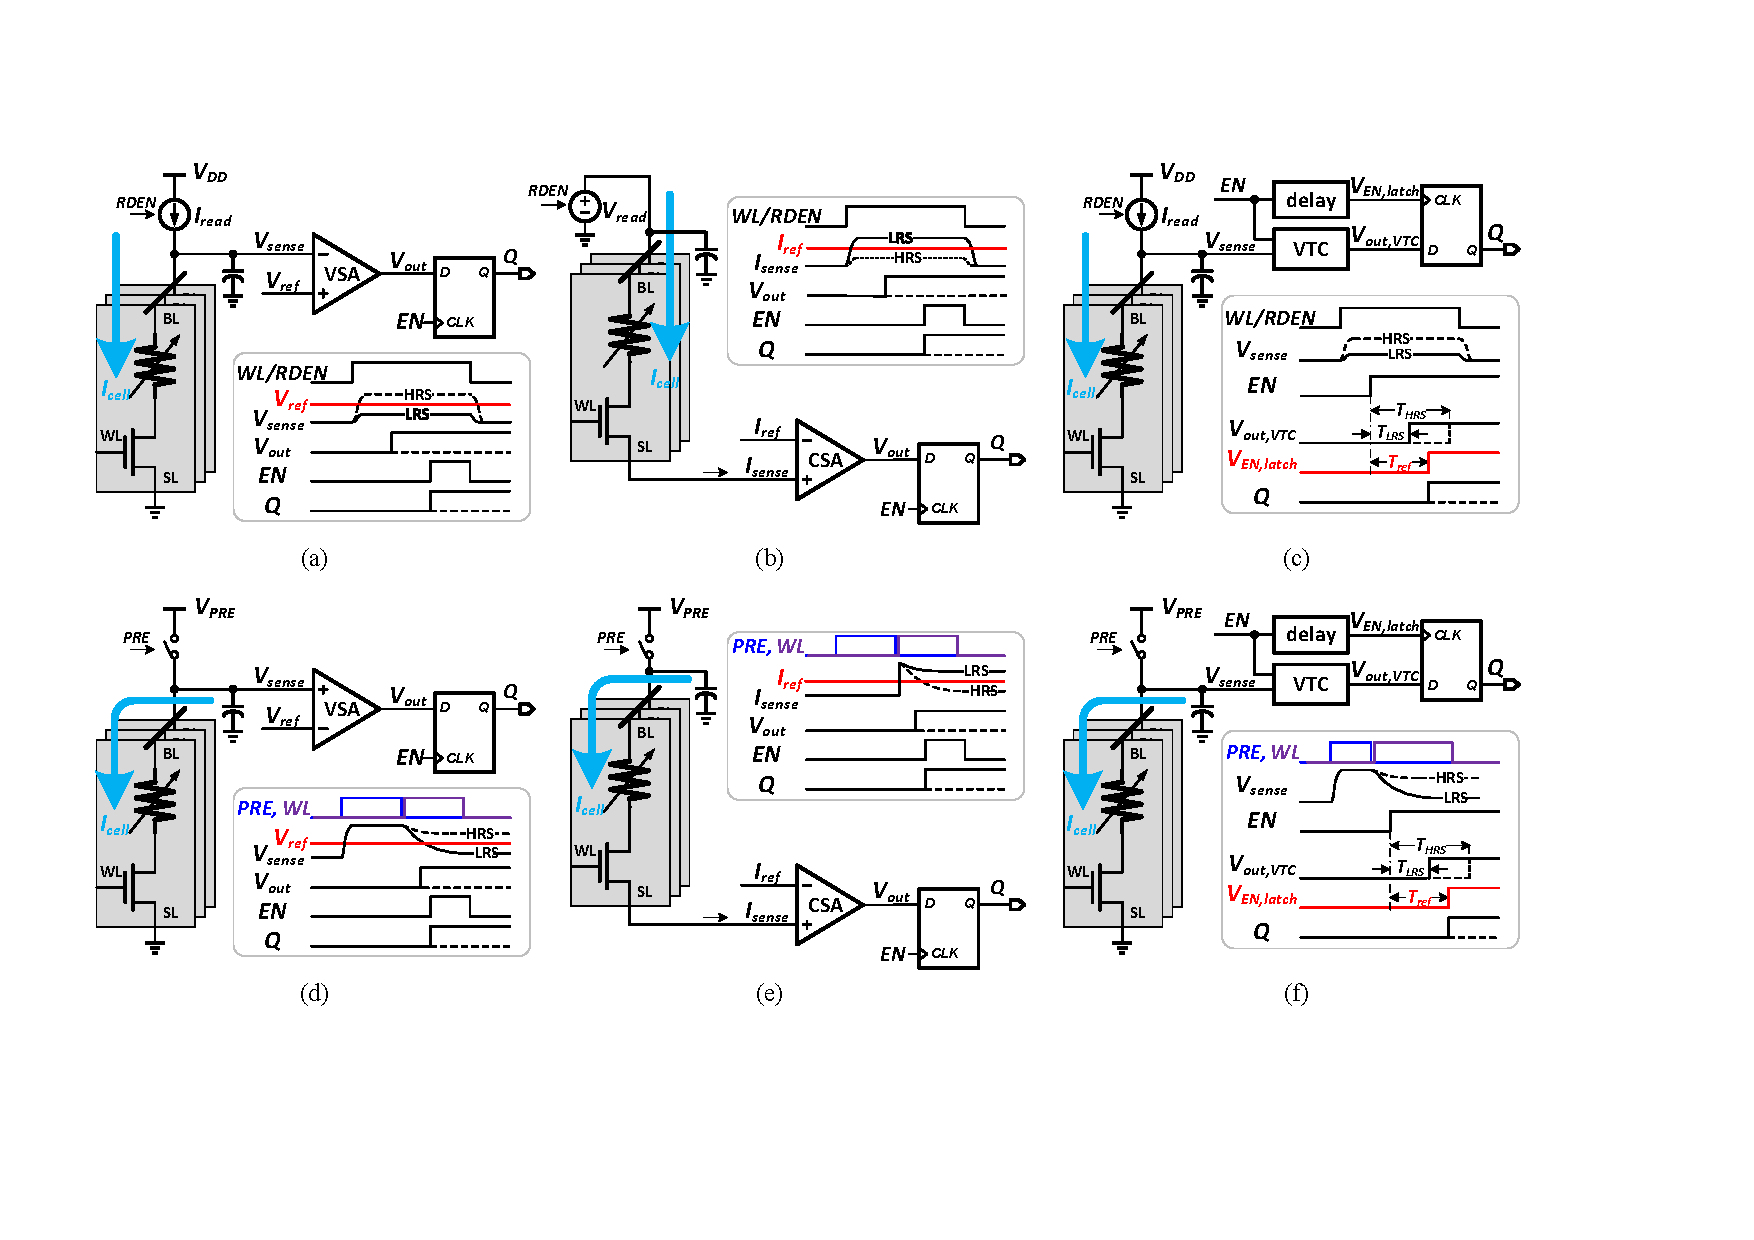
\includegraphics[width=0.95\textwidth]{fig/SA_types_new2.pdf}}
\caption{
The basic conceptual circuit schematics of three different sensing schemes for NVM array: (a) Voltage mode, (b) Current mode, and (c) Time mode w/o precharge process and (d) - (f) the above-mentioned sensing schemes w/ precharge process. 
Assuming one specific bitcell is selected.
}
\label{fig_sensing_mode}
\end{figure*}

\subsection{Prior Sensing Schemes of RRAM}

RRAM sensing is to convert the resistance state of the accessed RRAM bitcell into a digital value.
Because of the typical single-ended access operation, RRAM sensing schemes are different from conventional SRAM sensing but similar to DRAM sensing. 
% \st{Thanks to the feature of non-destructive reading under a reasonable read voltage, the sensing approaches of RRAM array are more flexible than that of conventional DRAM array.} 
Fig \ref{fig_sensing_mode} illustrates the operation principles of three main sensing modes (i.e., voltage mode, current mode, and time mode).

\subsubsection{Voltage Mode Sensing}
In the voltage mode sensing schemes \cite{yang20132mb, chang201419}, the bitcell voltage is sensed and compared with a reference voltage, which is a median value of an HRS cell and an LRS cell.
Fig. \ref{fig_sensing_mode}(a) illustrates the basic conceptual schematic of the voltage mode sensing for RRAM. The data stored in the bitcell is retrieved by forcing a fixed read current $I_{read}$ to the bit line (BL), and sensing the bit line voltage $V_{BL}$ by a voltage mode sense amplifier (VSA). 

\subsubsection{Current Mode Sensing} In the current mode sensing  \cite{jain201913, lo2018reram} (Fig. \ref{fig_sensing_mode}(b)), the data stored in the bitcell is retrieved by forcing a small fixed read voltage $V_{read}$ (smaller than the programming voltage so that the cell's state is not disturbed) to BL, and the 
%read current $I_{read}$ from source line is mirrored to compare
current through the bitcell is sensed and compared with a reference current $I_{ref}$ by a current mode sense amplifier (CSA). The reference current could be generated by two replica columns directly or by an extra reference generator circuit.

\subsubsection{Time Mode Sensing} Fig. \ref{fig_sensing_mode}(c) shows the operation of the time mode sensing \cite{trinh2018time}. 
The bitline voltage is converted into the time domain by a voltage-to-time converter (VTC) in the format of a long/short delay. A D-type flip-flop (DFF) serves as a time domain sense amplifier to compare the VTC result with an intrinsic delay that acts as a time domain reference. 
Once the enable signal $EN$ is activated, the VTC generates a signal $V_{out,VTC}$ with a time delay, depending on the input voltage $V_{sense}$, as illustrated in the timing diagram in Fig. \ref{fig_sensing_mode}(c). More specifically, an RRAM bitcell in LRS (HRS) determines a low (high) sense voltage $V_{sense}$, which generates a short (long) time delay $T_{LRS}$ ($T_{HRS}$) when a non-inverting VTC is assumed. The delay difference reflects the bitcell state, which is discriminated by the following DFF. Meanwhile, the enable signal generates a delayed signal $V_{EN,latch}$ by a delay chain with a fixed delay time $T_{ref}$ as the time domain reference, which is intermediate between $T_{LRS}$ and $T_{HRS}$. If the bitcell is in the LRS (HRS) state, the transition of $V_{out,VTC}$ will occur at $T_{LRS}<T_{ref}$ ($T_{HRS}>T_{ref}$), hence the latch will capture the high (low) logic level. As a result, the latch output indicates the bitcell state. 
% Ideally, the transition of $V_{EN,latch}$ occurs at $t_{ref}=$

In practice, however, the read operation is divided into three different phases -- precharging, developing, and sensing. BL is precharged to a precharge voltage $V_{PRE}$ before activating the word line (WL) and then kept floating. When activating WL, BL is discharged at different speeds according to the state of the cell. This developing phase is to obtain enough sensing margin. Then, a sense amplifier is enabled to detect the state.
Fig. \ref{fig_sensing_mode}(d)-(f) illustrate the above-mentioned three types of sensing schemes, where the current through the selected bitcell $I_{cell}$ is the discharge current drawing from the parasitic capacitor of bitline $C_{BL}$. The read energy can be reduced by precharging BL because the energy is only dissipated for charging the parasitic capacitor $C_{BL}$. While without precharging, the selected bitcell consumes extra energy as well during WL is activated.
% \textcolor{red}{Is it really necessary to precharge before sensing for NVM? YES!}

It should be noted that a latch (usually DFF) is necessary to hold the read-out value until the next read operation. This latch is usually driven by a read clock signal. For the time mode sensing, the DFF also acts as a sense amplifier, which compares the time delay of input signal $D$ and clock signal $CLK$.
Besides, an absolute reference voltage or current is required for voltage or current mode sensing while the time mode sensing is reference-less, simplifying the peripheral circuit design.
 As a result, the time mode sensing saves considerable area overhead compared with the conventional voltage mode and current mode sensing schemes.

\begin{figure}[!t]
\centerline
{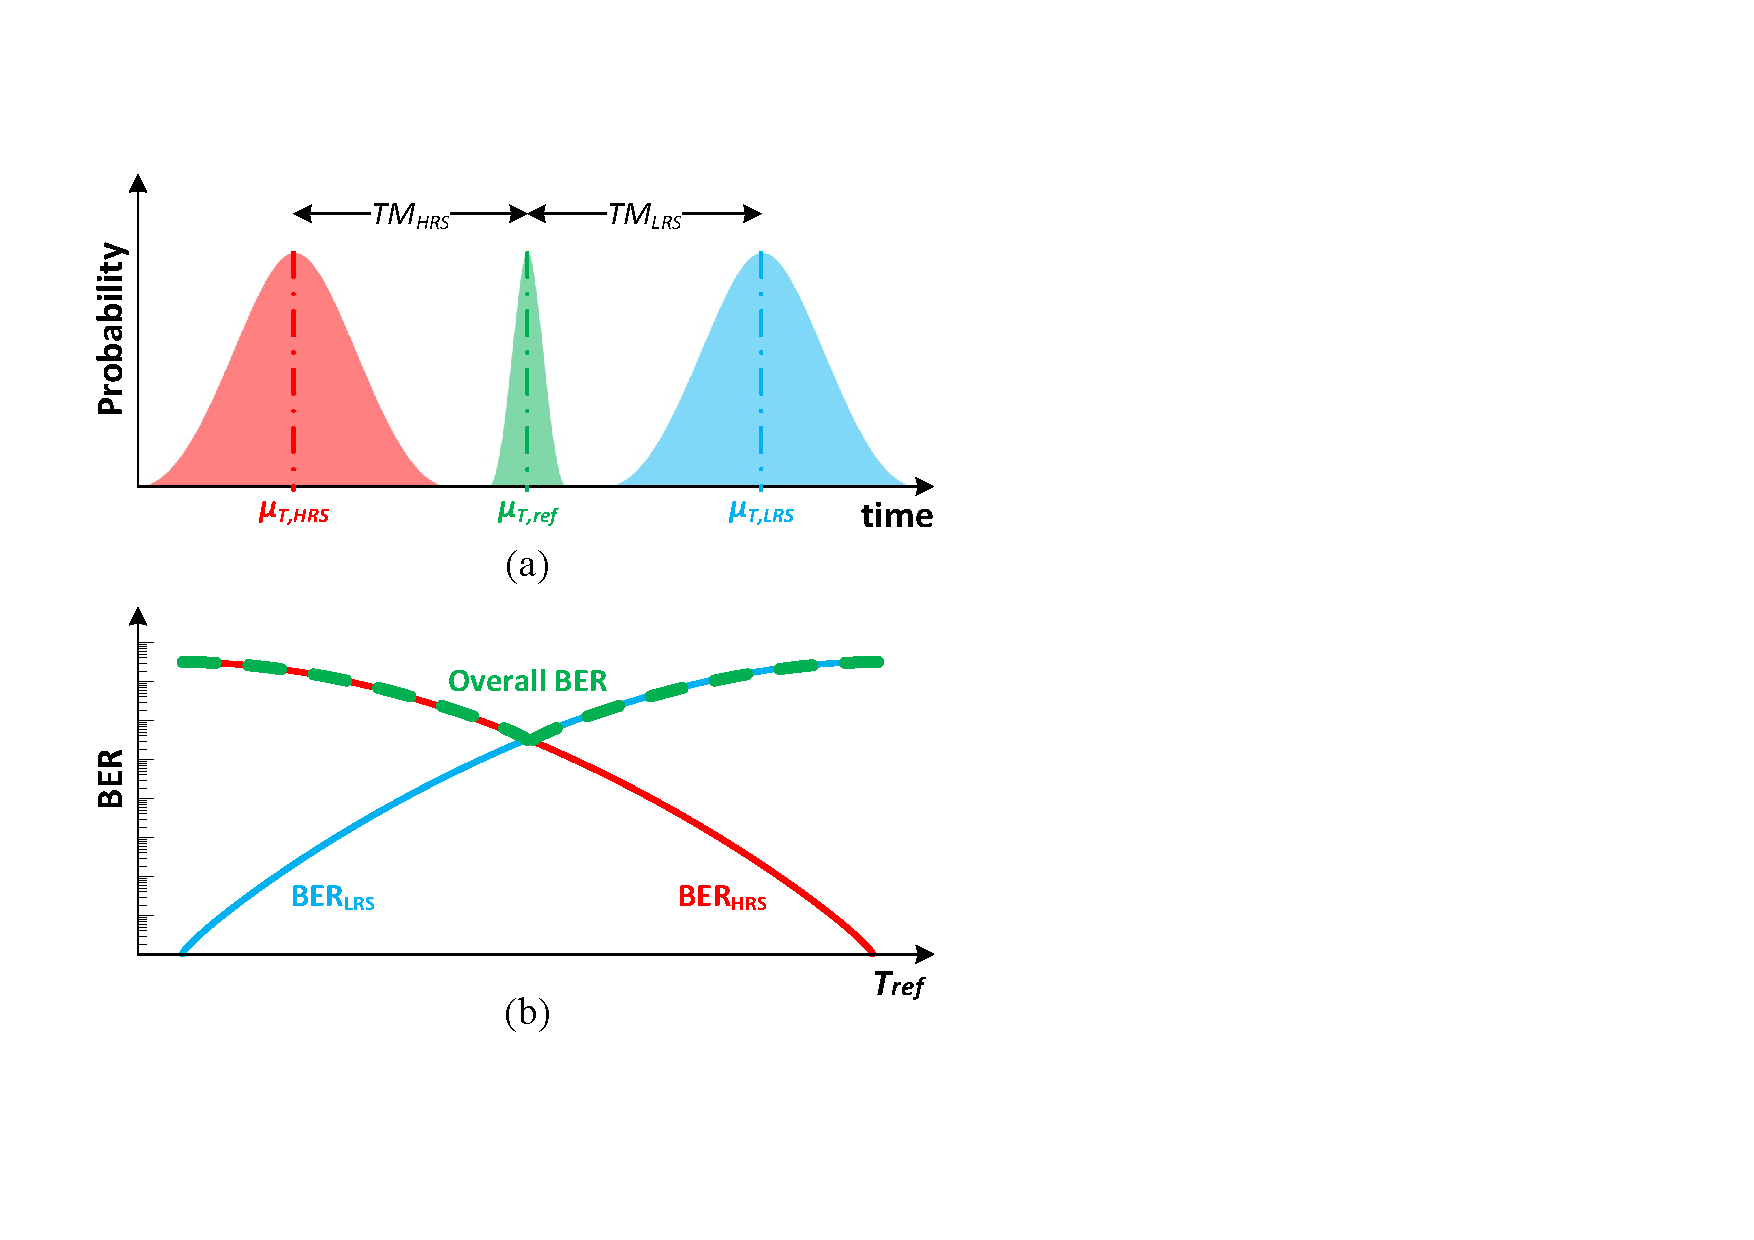
\includegraphics[width=0.42\textwidth]{fig/BER_probability.pdf}}
\caption{(a) Probability distribution of the time delay $T_{LRS}$, $T_{HRS}$ and time margin definition. (b) BER in LRS and HRS versus reference time $T_{ref}$ and the overall BER when optimizing $T_{ref}$.}
\label{fig_BER_probability}
\end{figure}

%% figure in the next section
\begin{figure*}[!t]
\centerline
{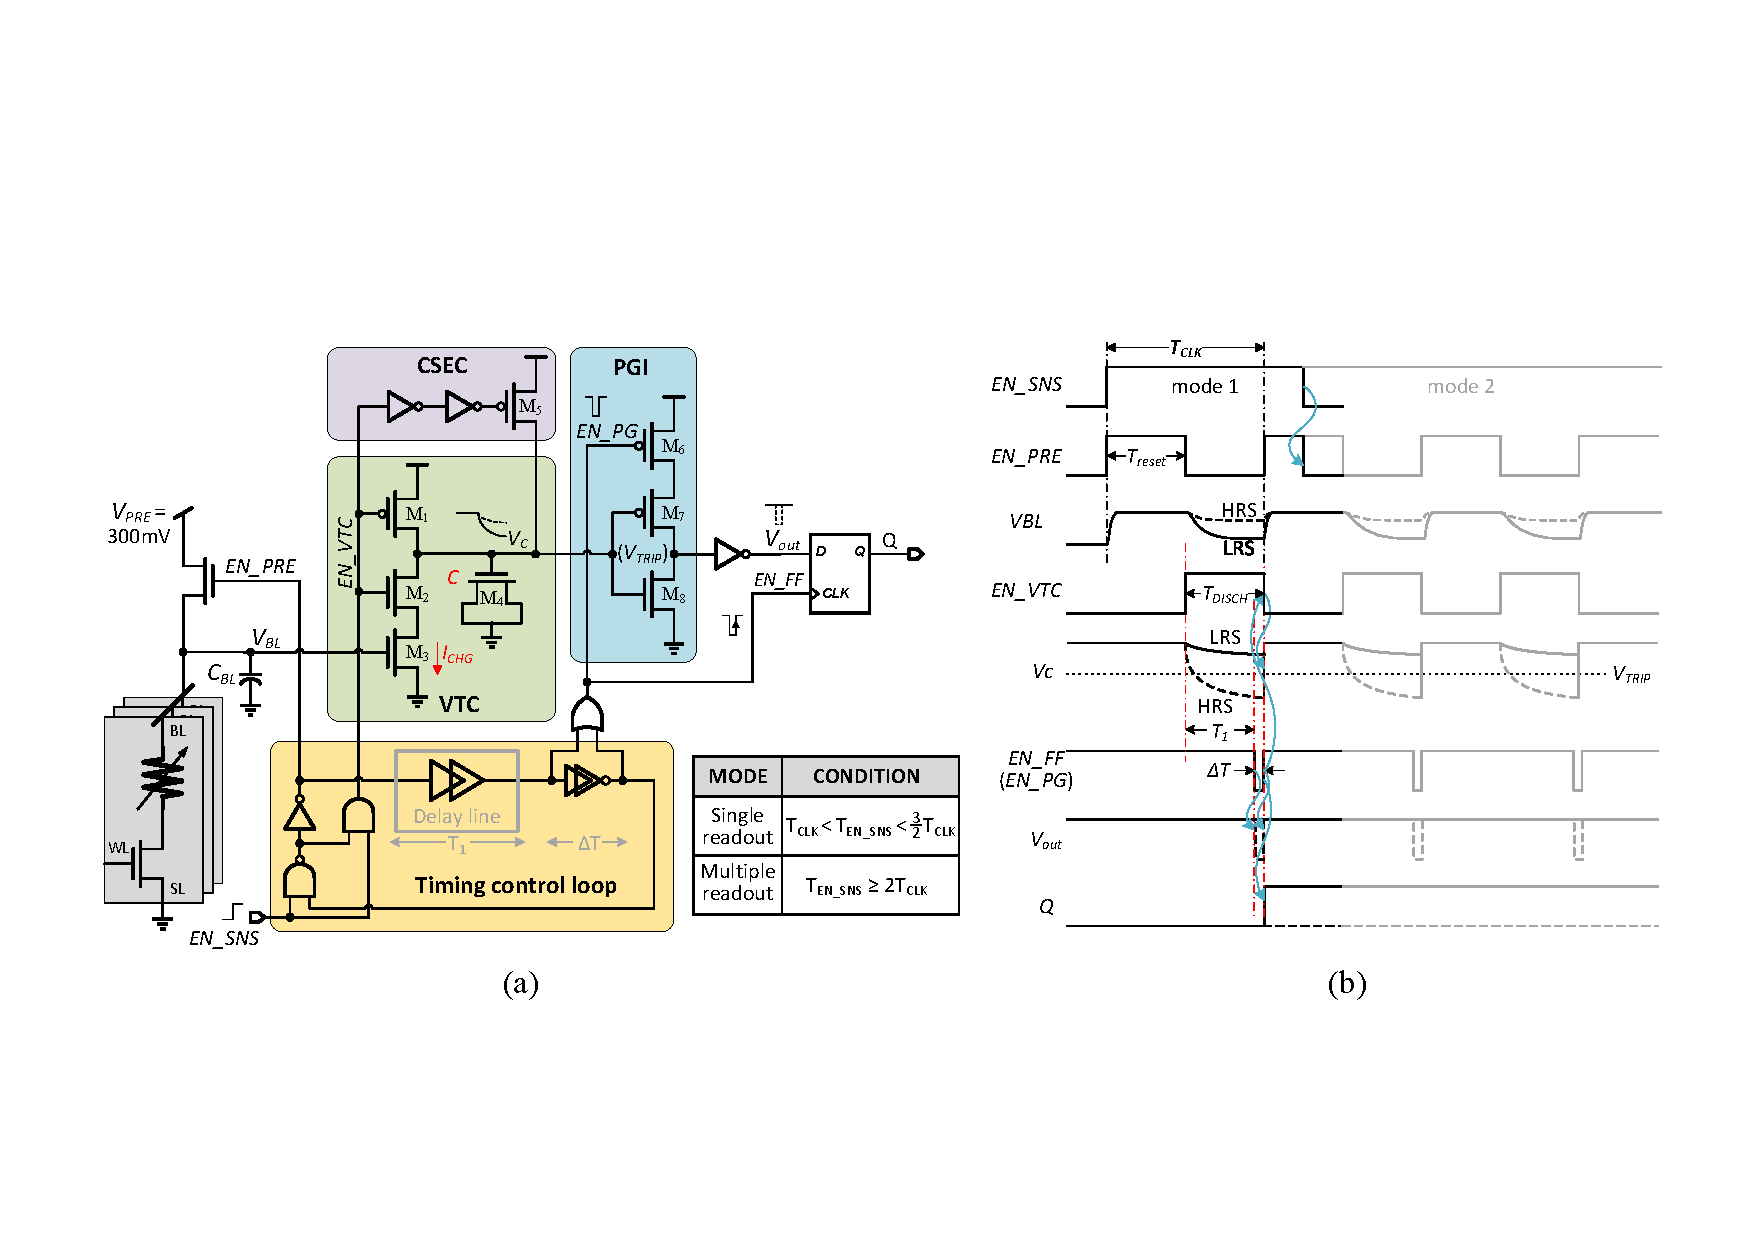
\includegraphics[width=0.97\textwidth]{fig/time_sensing_single.pdf}}
\caption{Proposed time-based single-level sensing: (a) circuit schematic that consists of voltage-time converter (VTC), power gating inverter (PGI), charge sharing-induced error compensation (CSEC) circuit, and time-domain controller. (b) Typical waveforms of critical nodes for different RRAM states (LRS and HRS) in different readout modes. }
\label{fig_prop_circuit}
\end{figure*}

\subsection{Challenges of Robust Sensing}
\label{challenges}

To enlarge the sensing margin and distinguish the resistance states reliably, higher bitline voltage $V_{BL}$ is desirable. However, the $V_{BL}$ must be kept considerably smaller than the typical program voltage to prevent read disturbance. This leads to an inevitable trade-off between read robustness and read disturbance.
Furthermore, random process variations degrade the sensing margins and increase read BER.

Fig. \ref{fig_BER_probability}(a) shows the probability distribution of the time delay at different states $T_{LRS}$ and $T_{HRS}$. 
The time domain reference $T_{ref}$ needs to be set appropriately to ensure adequate margin when variations are considered. 
Since the resistance of the RRAM is assumed to be Gaussian distributed \cite{6948806}, the time margin $TM_{LRS}=T_{LRS}-T_{ref}$ ($TM_{HRS}=T_{ref}-T_{HRS}$) can be represented as a random variable with the mean value $\mu_{TM,LRS}$ ($\mu_{TM,HRS}$) and the standard deviation $\sigma_{TM,LRS}$ ($\sigma_{TM,HRS}$). 
Ideally, the transition of $V_{EN,latch}$ occurs at $T_{ref}=\frac{1}{2}(T_{LRS}+T_{HRS})$ to maximize the time margin $TM$ ($TM=min	\left\{TM_{LRS}, TM_{HRS}\right\}$) and minimize the read BER.
Setting the reference time $T_{ref}$ away from $T_{LRS}$ will reduce $BER_{LRS}$ but increase $BER_{HRS}$, and vice versa, as illustrated in Fig. \ref{fig_BER_probability}(b).
The BER in LRS (HRS) is the probability that the time margin $TM_{LRS}$ ($TM_{HRS}$) is negative, which is given by \cite{trinh2018time}
\begin{align}
\label{eq_ber}
BER_X &= {\rm Pr}[TM_X<0] \notag \\
      &= \frac{1}{2}\left[1+{\rm erf}\left(\frac{-1/\sqrt{2}}{\sigma_{TM,X}/\mu_{TM,X}}\right)\right]
\end{align}
% \begin{align}
% \label{eq_ber}
% BER_X = Pr[TM_X<0] 
%       = \frac{1}{2}[1+erf(\frac{1}{\sqrt{2}} \frac{1}{\sigma_{TM,X}/\mu_{TM,X}})]
% \end{align}
where the subscript $X$ stands for the state of the bitcell (either LRS or HRS), and erf is the Gaussian error function \cite{walpole1993probability}. 
From \eqref{eq_ber}, the read robustness against variations depends only on the sensing margin variability $\sigma_{TM,X}/\mu_{TM,X}$.
For example, a sensing margin variability of 0.21 (0.167) leads to a BER of $10^{-6}$ ($10^{-9}$).
As expected, lower variability in the sensing margin achieves better (i.e., lower) read BER. 

The overall BER is determined by the worst case between LRS and HRS in Eq. \eqref{eq_ber}. 
The sensing margin is limited because (a) the voltage or current applied to the bitcell is small to avoid disturbing, and (b) the resistance ratio is not high enough considering variations.
It is noted that in the worst case where the LRS and HRS values are overlapped (i.e., $R_{LRS}>R_{HRS}$), the states are indistinguishable, and hence it is impossible to read the bitcell correctly. 


